\subsubsection{Descrizione}

In questo modulo, chiamato \textbf{Front-end\ped{G}}, viene gestita la parte visibile del sito \nameproject{} e come essa interagisce con l'utente ed il modulo \textbf{Back-end\ped{G}}. L'architettura generale del modulo è basata su pattern offerti da Next.js\ped{G} e React\ped{G}. In particolare vengono utilizzati:
\begin{itemize}
	\item \textbf{Presentational and Container component pattern}: suddivisione dei component in viste e loro relativa logica;
	\item \textbf{Observer pattern}: rendering della view in seguito al cambiamento di stato.
\end{itemize} 
Questi saranno spiegati in modo più approfondito nella sezione \S{2.2.5}.\\
Il modulo \textbf{Front-end\ped{G}} interagisce con il modulo \textbf{Back-end\ped{G}} attraverso delle API\ped{G} esposte dal servizio Amazon API Gateway e chiamate dal nostro package\ped{G} Services, che è composto da funzioni che gestiscono l'interazione e la risposta di esse. \\
Di seguito viene mostrata un'architettura generale che rappresenta come il modulo opera ad alto livello.

\vspace{1cm}

\begin{figure}[H]
\centering
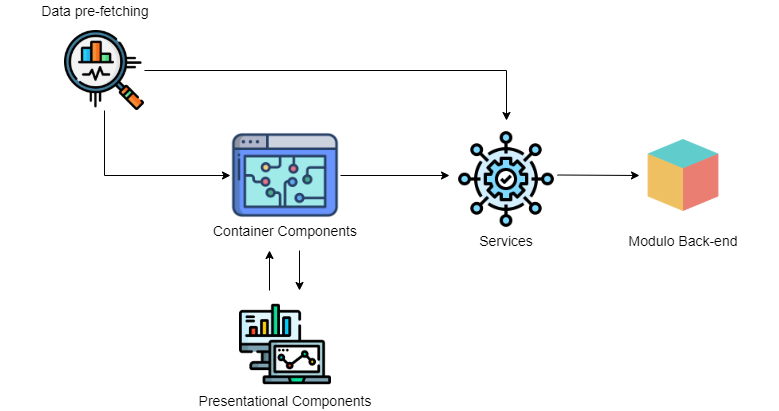
\includegraphics[scale=0.48]{res/Architettura/Frontend/img/general_frontend}\\
\caption{Schema generale del modulo Front-end\ped{G}}
\end{figure}